On the domain of figure~\ref{40000029:domain}, the differential equation
\[
\Delta u = \lambda u
\]
is to be solved with homogeneous boundary conditions.
Reduce this problem to the solution of two ordinary differential equations
with boundary conditions and solve at least one of them.
\begin{figure}[h]
\centering
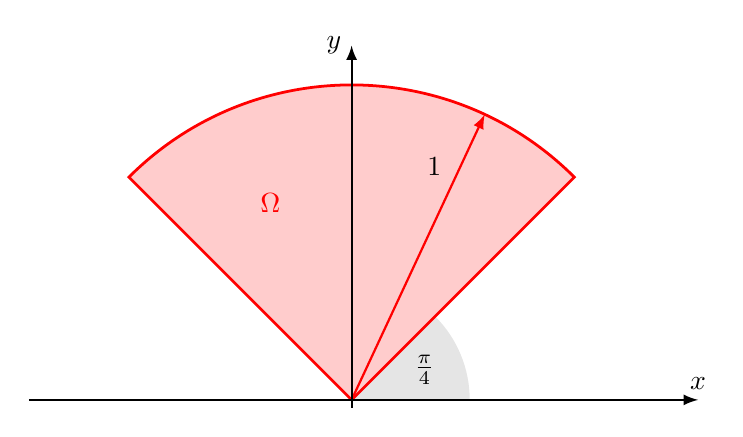
\begin{tikzpicture}[>=latex,thick]
\fill[color=gray!20] (0,0) -- (0:1.5) arc (0:45:1.5) -- cycle;
\node at (22.5:1) {$\frac{\pi}4$};
\fill[color=red!20] (0,0) -- (45:4) arc (45:135:4) -- cycle;
\node[color=red] at (112.5:2.7) {$\Omega$};
\draw[color=red,line width=1pt] (0,0) -- (45:4) arc (45:135:4) -- cycle;
\draw[->,color=red] (0,0) -- (65:4);
\node at (65:3) [above left] {$1$};
\draw[->] (-4.1,0) -- (4.4,0) coordinate[label={$x$}];
\draw[->] (0,-0.1) -- (0,4.5) coordinate[label={left:$y$}];
\end{tikzpicture}
\caption{Domain for the operator in problem~\ref{40000029}
\label{40000029:domain}}
\end{figure}

\begin{hinweis}
Note that linear combinations of sine and cosine functions can
always be written as a phase shifted sine function:
\[
A\cos \alpha + B \sin \alpha =  C \sin(\alpha+\delta).
\]
\end{hinweis}

\begin{loesung}
In polar coordinates, the domain is described as
\[
0< r < 1
\qquad\text{and}\qquad
\frac{\pi}4 < \varphi < \frac{3\pi}{4},
\]
which lends itself to solution using a separation ansatz
$u(r,\varphi) = R(r)\Phi(\varphi)$.
The Laplace operator in polar coordinates is
\[
\Delta
=
\frac1r \frac{\partial}{\partial r}r\frac{\partial }{\partial r}
+
\frac1{r^2}\frac{\partial^2}{\partial r^2}.
\]
Using the ansatz, we get
\[
\Delta u
=
\frac{1}{r}\frac{\partial}{\partial r} rR'(r)\Phi(\varphi)
+
\frac{1}{r^2}R(r)\Phi''(\varphi)
=
\frac{1}{r}(R'(r)+rR''(r))\Phi(\varphi)
+
\frac{1}{r^2}R(r)\Phi''(\varphi)
=
-\lambda R(r)\Phi(\varphi)
\]
Dividing by $u(r,\varphi)$ and multiplying by $r^2$ gives
\[
\frac{rR'(r)+r^2R''(r)+\lambda r^2R(r)}{R(r)}
+
\frac{\Phi''(\varphi)}{\Phi(\varphi)}
=
0.
\]
This allows to separate the variables $r$ and $\varphi$, giving
\[
\frac{rR'(r)+r^2R''(r)+\lambda r^2R(r)}{R(r)}
=-
\frac{\Phi''(\varphi)}{\Phi(\varphi)}
\;\Rightarrow
\left\{
\;
\begin{aligned}
rR'(r)+r^2R''(r)+\lambda r^2R(r) &= \mu R(r) \\
\Phi''(\varphi) &= -\mu \Phi(\varphi).
\end{aligned}
\right.
\]
The boundary conditions are
\begin{equation}
\Phi\biggl(\frac{\pi}4\biggr)=\Phi\biggl(\frac{3\pi}4\biggr)=0 
\qquad\text{and}\qquad
   R(0)=R(1)= 0.
\end{equation}
The $\Phi$-equation is a harmonic oscillation, so the solution must be
\[
\Phi(\varphi)
=
A \cos\sqrt{\mu}\varphi + B \sin\sqrt{\mu}\varphi
=
C\sin(\sqrt{\mu}\varphi + \delta).
\]
At the boundary $\varphi=\frac{\pi}4$, we have
\[
0
=
\Phi\biggl(\frac{\pi}4\biggr)
=
C\sin\biggl(\sqrt{\mu}\frac{\pi}4+\delta\biggr)
\]
with the solution $\delta=-\sqrt{\mu}\frac{\pi}4$.

At the boundary $\varphi=\frac{3\pi}4$ we get
\[
\Phi\biggl(\frac{3\pi}4\biggr)
=
C\sin\biggl(\sqrt{\mu}\frac{3\pi}4-\sqrt{\mu}\frac{\pi}4\biggr)
=
C\sin\sqrt{\mu}\frac{\pi}{2}
=
0
\quad\Rightarrow\quad
\frac{\sqrt{\mu}}2 \in \mathbb{N}
\quad\Rightarrow\quad
\mu = 4k^2,\;k\in\mathbb{N}.
\]
This means that $R_k(r)$  must be a solution
\[
r^2R''(r) + rR'(r) +(\lambda r^2-4k^2) R(r) = 0.
\]
This is the Bessel equation which can be solved using Bessel functions.
\end{loesung}

\begin{bewertung}
Separation ansatz ({\bf A}) 1 point,
equation for $R(r)$ ({\bf R}) 1 point,
boundary conditions for $R(r)$ ({\bf B}) 1 point,
equation for $\Phi(\varphi)$ with boundary conditions ($\Phi$) 1 point,
solution for $\Phi(\varphi)$ ({\bf S}) 1 point,
admissible values of $\mu$ ({\bf M}) 1 point.
\end{bewertung}
